
\subsection{1.28 Клиновидные сэндвичевые соединения переходных металлов (гомолигандные, гетеролигандные). Способы получения и условия стабильности, геометрия, электронное строение, свойства.}
\begin{figure} [H]
	\centering {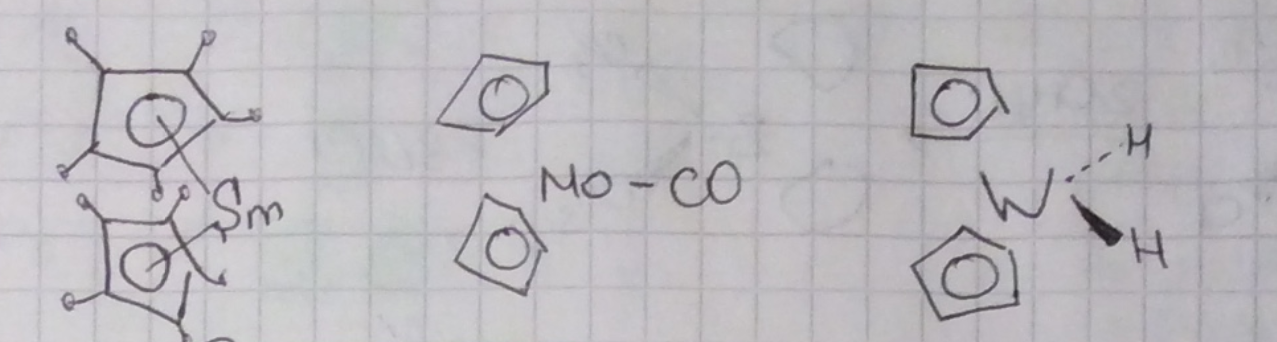
\includegraphics[scale=0.6]{ss1}}
\end{figure}
С объемными $M$, с дополнительными лигандами $(-H, -CO, ...)$
\textbf{Способы получения:}\\
\begin{figure} [H]
	\centering {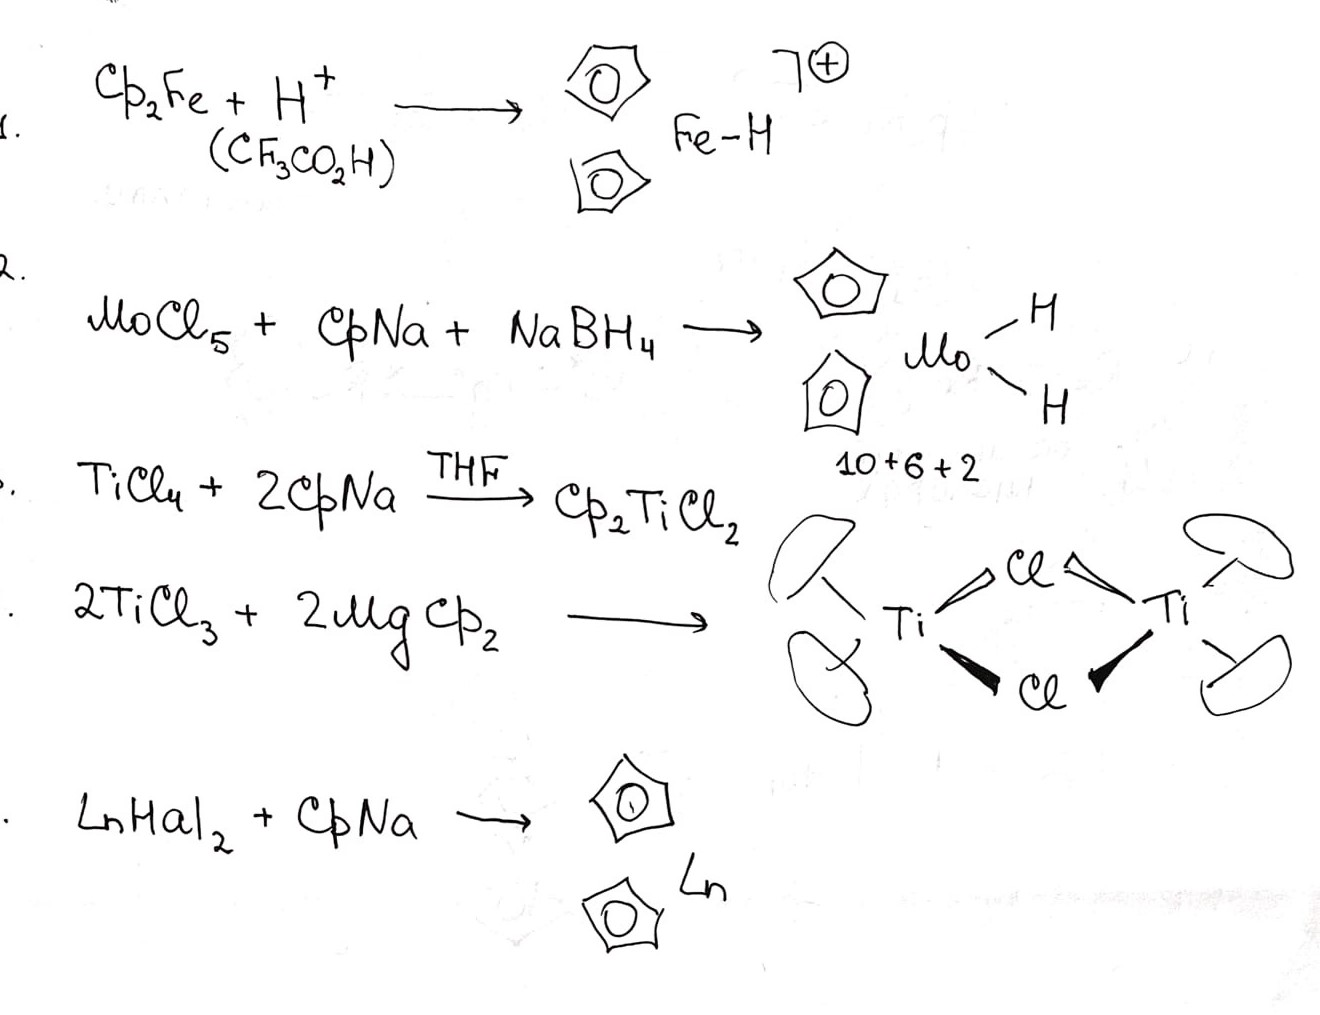
\includegraphics[scale=0.4]{ss2}}
\end{figure}
\textbf{Условия стабильности}\\
18 электронов \\
\textbf{Свойства}\\
\begin{figure} [H]
	\centering {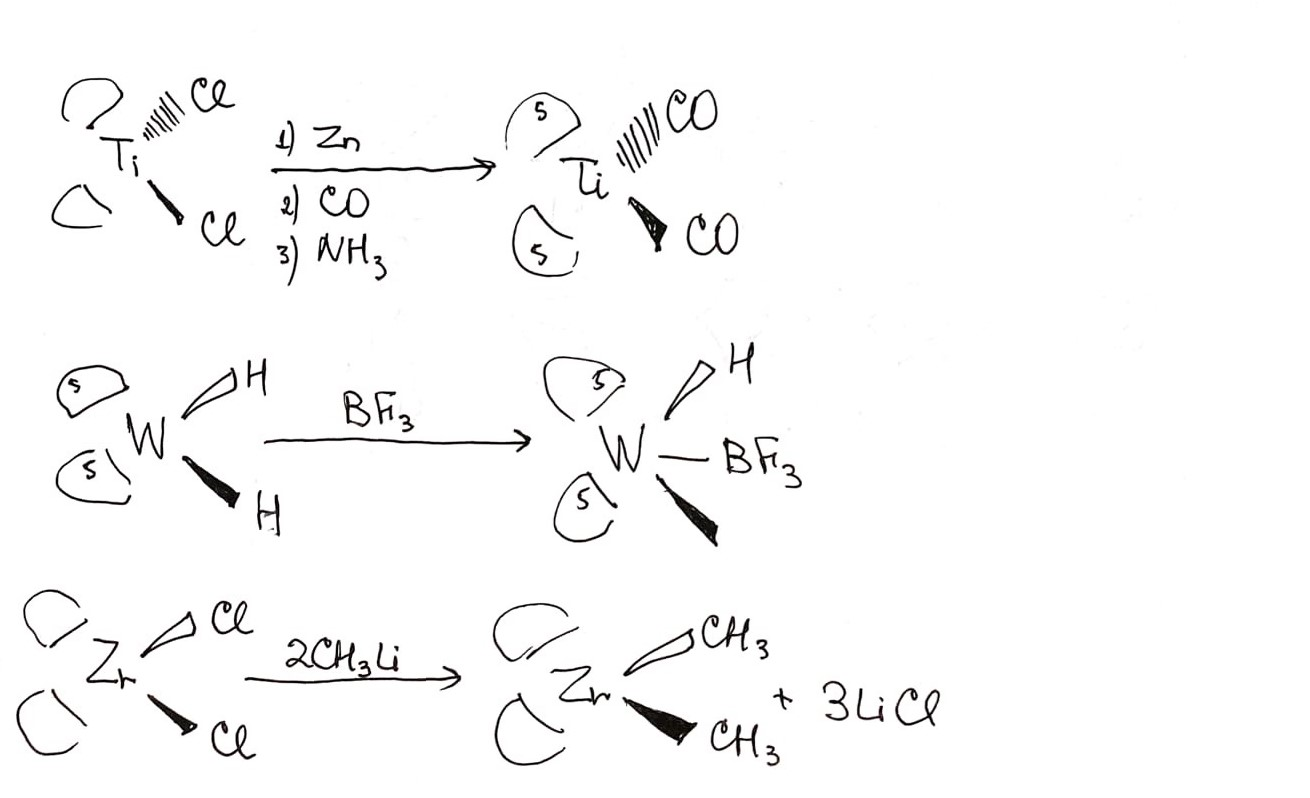
\includegraphics[scale=0.4]{ss3}}
\end{figure}
